\documentclass[fleqn,usenatbib]{mnras}

\usepackage{amsmath}	% Advanced maths commands
\usepackage{graphicx} % Required for inserting images
\usepackage{booktabs} % For better table formatting
\usepackage{xcolor}
\graphicspath{ {./plots/} }

\newcommand{\kms}{\,km\,s$^{-1}$} % kilometres per second
\newcommand{\bibtex}{\textsc{Bib}\!\TeX}

\newcommand{\dstn}[1]{{\color{teal}{#1}}}
\newcommand{\todo}[1]{{\color{red}{[TODO: #1]}}}
\newcommand{\figtodo}[1]{\fbox{\parbox{0.45\textwidth}{\centering\vspace{2em}{\color{red}Figure to be generated:}\\ #1\vspace{2em}}}}

\bibliographystyle{mnras}

\title[Proper Motions and Parallaxes in DESI Imaging]{Proper Motions and Parallaxes of Stars in the DESI Legacy Imaging Surveys}

\author[Nada El-Falou et al.]{
Nada El-Falou,$^{1, 2}$\thanks{E-mail: nelfalou@uwaterloo.ca}
Dustin Lang$^{2}$
\\
% List of institutions
$^{1}$Waterloo Center for Astronomy, Department of Physics and Astronomy, University of Waterloo, \\
\hspace{0em} 200 University Avenue West, 
Waterloo, ON, N2L 3G1, Canada \\
$^{2}$Perimeter Institute for Theoretical Physics, 
31 Caroline Street North,
Waterloo, ON, N2L 2Y5, Canada \\
}

\date{January 2025}

\begin{document}
\label{firstpage}
\pagerange{\pageref{firstpage}--\pageref{lastpage}}
\maketitle

% \begin{abstract}
% I did this and that, resulting in that and this.
% \end{abstract}

% Select between one and six entries from the list of approved keywords.
% Don't make up new ones.

% \begin{keywords}
% keyword1 -- keyword2 -- keyword3
% \end{keywords}


\section{Introduction}

By measuring the positions, brightnesses and motions of stars, we can map out the Milky Way, study its stellar dynamics, and trace its history. Learning the trajectories of stars can also reveal their gravitational interactions with massive systems that may or may not be visible, like black holes and dark matter. We can find patterns in the stars' motions that reveal systems such as globular clusters' tidal tails, which can constrain properties of the Milky Way and surrounding dwarf galaxies.   High-velocity stars, such as hyper-velocity stars, runaway stars, hyper-runaway stars, and fast halo stars, can be used to probe the physical processes and systems responsible for propelling them. In short, proper motions and parallaxes contribute to everything from constructing accurate maps of our Galaxy to uncovering hidden structures.


% High-velocity stars, encompassing a variety of types such as hyper-velocity stars, runaway stars, hyper-runaway stars, and fast halo stars, offer valuable insights into the intricate physical processes and systems responsible for propelling these celestial bodies. Exploring the characteristics and origins of these high-velocity stars unveils a wealth of knowledge about the underlying mechanisms shaping their trajectories.

% High-velocity stars serve as unique tools for probing the Milky Way, traversing the galaxy during their lifetimes and offering insights into some of the universe's most extreme phenomena \citep{Marchetti2021}. Two primary mechanisms contribute to the ejection of young O- and B-type stars at high Galactic latitudes: the explosion of a supernova in a binary system and close encounters in dense stellar systems. While the majority of runaway stars exhibit velocities below ~10 km/s (referred to as walkaway stars), some can attain speeds up to several hundred km/s, with predicated upper limits around 450 km/s \citep{Marchetti2021}.

% Hyper-runaway and hypervelocity stars, in particular, provide a window into stellar evolutionary processes, such as the impact of natal kicks on neutron stars and other compact objects \citep{Igoshev2022}. Binary evolution processes, including supernova kicks in binaries, can eject companions of exploding stars at velocities comparable to orbital speeds at the point of explosion. Additionally, stellar dynamical processes within collisional cluster environments may lead to hyper-runaway ejections. Intriguingly, interactions with massive black holes could result in the emergence of extreme hyper-velocity stars, reaching speeds of hundreds or even thousands of kilometers per second \citep{Igoshev2022}.

% Hypervelocity stars, distinguished by their extremely high velocities in the order of thousands of km/s, present an intriguing phenomenon \citep{Marchetti2021}. These velocities are often achieved through close interactions between binary systems and the massive black hole residing in the Galactic Center. Hypervelocity stars serve as valuable tools for probing the shape and orientation of matter, including dark matter, distribution in the Galaxy. Various ejection mechanisms contribute to the formation of hypervelocity stars, such as runaway stars and hypervelocity stars from the Large Magellanic Cloud, acceleration of single stars following interactions between a black hole binary and Sagittarius A*, tidal interactions of dwarf galaxies with the Milky Way, and the infall of dwarf galaxies toward the Galactic Center \citep{Marchetti2021}.

%%%%%%%%%%%%%% My notes:
% High-velocity stars, including hyper-velocity stars, runaway stars, hyper-runaway stars, and fast halo stars, provide valuable insights into the physical processes and systems that accelerated those stars.

% - About hyper-runaway and hypervelocity stars: "These include stellar evolutionary processes like natal kicks given to neutron stars and possibly other types of compact objects; binary evolution processes, such as supernova kicks in binaries, ejecting the companion of the exploding stars at velocities comparable to the orbital velocities at the point of explosion, remnants of Ia/Iax supernova explosion; and stellar dynamical processes in collisional cluster environments, where few-body interactions can give rise to hyper-runaway ejections; or through dynamical interaction with massive black holes that may even give ruse ti extreme hyper-velocity stars ejected at hundreds or thousands km/s" \citep{Igoshev2022}. 

% - About general high velocity: These stars "are unique tools to probe our Milky Way: they travel through the galaxy during their lifetime, being observed far way from their birthplace, and they give us insight into some of the most extreme phenomena in our universe" ... The two main ejection mechanisms of young O- and B-type stars at high Galactic latitude, runaway stars, are "the explosion of the supernova in a binary system, with the companion star being ejected with a high velocity;" and close encounters in dense stellar systems."... "The majority of runaway stars produced by both scenarios have typical velocities below ~10 km/s, the so-called walkaway stars."... "velocities up to several hundreds of km/s can be attained"..."predicated upper limits are around 450 km/s" ... \citep{Marchetti2021}

% - About hypervelocity stars: "Extremely high velocities of order thousands of km/s can instead be easily reached by hypervelocity stars (HVSs)... as a result of a close interaction between a binary system and the massive black hole residing in the Galactic Centre."HVSs [can be] used as tools to probe the shape and orientation of matter (and dark matter) distribution in the Galaxy." ... "Other ejection mechanisms ... runaway stars and HVSs from the Large Magellanic Cloud, the acceleration of single stars following the interaction between a black hole binary made of Sagittarius A* and an intermediate mass black hole, tidal interactions of dwarf galaxies with the Milky Way, and the infall of dwarf galaxies towards the Galactic Centre." \cite{Marchetti2021}

\section{Existing Data}
Astronomical surveys have historically provided essential data by compiling precise measurements of stellar positions and motions. Each survey has its strengths and limitations, depending on its target, observing techniques, and instrumental sensitivity. Here, we review several foundational surveys, highlighting their contributions and limitations to contextualize our new dataset.

The Hipparcos satellite, launched by ESA, was groundbreaking as the first dedicated astrometry mission, offering proper motions and parallaxes for over 100,000 stars. This dataset, however, was limited to relatively bright stars, with uncertainties rising significantly for fainter objects near its detection limit of \( V \approx 12 \) mag \citep{HIPPARCOS_1997}. %Following this, the Gaia mission has transformed astrometry with precision down to 0.02 mas for over a billion stars up to \( G \approx 21 \) mag in its third data release (DR3), providing an extensive view of stellar motion in the Milky Way \citep{GaiaDR2, GaiaDR3}.

Ground-based optical surveys, such as the Sloan Digital Sky Survey (SDSS) and Pan-STARRS, have contributed significantly to astrometry and photometry with observations in the g, r, i, and z bands. These surveys offer deep observations down to $g \sim 23.5$ mag (SDSS) and $g \sim 23.3$ mag (Pan-STARRS), enabling the detection of faint stars and other celestial objects \citep{SDSS_2000, PanSTARRS_2016}. However, SDSS only performed single-pass observations, meaning that it did not provide proper motion measurements for most of its sources, except in the Stripe 82 region, where multiple observations were taken, allowing for proper motion studies \citep{SDSS_2000}. %However, ground-based observations are inherently affected by atmospheric interference, which limits astrometric precision compared to space-based missions. Furthermore, these surveys primarily avoid dusty Galactic plane regions due to significant extinction and focus on areas with less obscuration.


Infrared surveys, such as the VISTA Hemisphere Survey (VHS), UKIRT Infrared Deep Sky Survey (UKIDSS), and Two Micron All-Sky Survey (2MASS), provide important data for studying stars obscured by dust. VHS reaches detection limits of $K \sim 20$ mag \citep{VHS}. UKIDSS achieves similar depths in its various sub-surveys \citep{UKIDSS_2007}. In contrast, 2MASS, which prioritized all-sky coverage over depth, has limits of $K \sim 14$ mag \citep{2MASS_2003}. However, the lower resolution and sensitivity of these infrared surveys, compared to optical surveys, restrict their precision, particularly for faint objects.

Finally, future observations with the Vera Rubin Observatory and the Legacy Survey of Space and Time (LSST) promise to bridge several of these gaps by observing faint stars with frequent revisits across the southern sky. LSST will provide exceptional temporal coverage for proper motion studies but will still face challenges observing obscured or highly reddened regions in the galactic plane \citep{Rubin2019}.

\begin{table*}
    \centering
    \caption{Summary of notable astronomical surveys and their properties. The DESI Legacy Surveys, which include data from the DECam instrument, observe in the optical  bands. Depth type refers to whether data is based on single-visit observations (one exposure per field) or coadded images (combined exposures to improve depth). Astrometric precision  is given in milliarcseconds (mas).}
    \label{tab:wide_table}
    \begin{tabular}{lcccccccc}
    \toprule
    Survey & Num objects (million) & $\lambda$ & Max mag & $\sigma_{\mu}$ (mas\,yr$^{-1}$) & Baseline (yrs) & Sky Coverage (deg$^2$) & Reference \\
    \midrule
    Hipparcos & 0.118 & Optical (V) & \( V \approx 12.4 \) & 1--2 & 4 & $\sim 40,000$ (all-sky) & \cite{HIPPARCOS_1997} \\ 
    SDSS Stripe 82 & 300 & Optical (ugriz) & \( r \approx 24.6 \) & $\sim 5$ & 10 & $\sim 300$ & \cite{SDSS_2000} \\
    Pan-STARRS & 3,000 & Optical (grizy) & \( i \approx 23.3 \) & $\sim 3$--10 & 4 & $\sim 30,000$ & \cite{PanSTARRS_2016} \\
    2MASS & 470 & NIR (JHK) & \( K \approx 14 \) & $\sim 10$ & 1 & $\sim 40,000$ (all-sky) & \cite{2MASS_2003} \\ 
    UKIDSS & 1,000 & NIR (YJHK) & \( K \approx 18.3 \) & $\sim 10$ & 7 & $\sim 7,500$ & \cite{UKIDSS_2007} \\
    VHS & 500 & NIR (JHKs) & \( K \approx 20 \) & $\sim 10$ & 5 & $\sim 20,000$ & \cite{VHS} \\
    Gaia EDR3 & 1,800 & Optical (G) & \( G \approx 21 \) & 0.01--0.5 & 2.5 & $\sim 40,000$ (all-sky) & \cite{GaiaEDR3} \\
    DECam & 1,000 & Optical (grz) & \( z \approx 23.0 \) & \todo{measured} & 6 & $\sim 14,000$ & \cite{legacy2019} \\
    \bottomrule
\end{tabular}


    
\end{table*}

\subsection{Gaia}
The Gaia mission, launched by the European Space Agency (ESA) in December 2013, is a groundbreaking space observatory designed to chart a three-dimensional map of our galaxy, the Milky Way, with unprecedented precision. By continuously scanning the sky from its vantage point at the L2 Lagrange point, Gaia collects astrometric, photometric, and spectroscopic data, enabling detailed analysis not only of stars but also of exoplanets, asteroids, and distant galaxies. The third early data release (EDR3) provides proper motion data for $1.8$ billion sources brighter than $g \sim 21$ mag \citep{GaiaDR3}, with precision down to $0.02$ mas. 

% Gaia DR3 introduces additional features such as mean radial velocities for over 33 million objects, low-resolution BP/RP spectra, and astrophysical parameters for 470 million sources \citep{GaiaDR3}. It also includes detailed variability analysis, orbital elements for binary systems, and new discoveries among Solar System objects. The release incorporates the Gaia Andromeda Photometric Survey, covering sources within a 5.5-degree radius of the Andromeda galaxy.

For our study, Gaia’s precise astrometry and photometry serve as a ``ground-truth" reference for calibrating and correcting proper motion and parallax measurements derived from DESI Legacy Imaging Survey data, extending these measurements to sources several magnitudes fainter than the Gaia limit. \todo{quote the faint limit at which our PM precision becomes uninformative, from the precision-vs-magnitude figure}

\dstn{(I think you could add the plot showing how we see this data product adding value to Gaia -- the plot showing the Gaia uncertainties on RA,Dec versus magnitude, and the Legacy Surveys plot showing the same.  You can then point out: (a) at the Gaia limiting mag, the LS positional errors are worse, but (b) the Legacy Surveys go a couple of mags deeper; but also (c) the LS quoted uncertainties are only \emph{statistical} uncertainties, omitting \emph{systematic} uncertainties -- which really was the majority of your effort on this project.)
}

\subsection{DESI Legacy Imaging Surveys} \label{Legacy data}
%The Legacy Surveys \citep{legacy2019}, which form the basis of our proper motion catalog, observe in the  bands using silicon CCDs. Although bands technically extend into the near-infrared, they are grouped with the optical range as a result of their use of CCD technology. These surveys avoid regions of high dust extinction, such as the Galactic plane, and thus do not significantly benefit from reduced dust obscuration. The primary advantage of the Legacy Surveys lies in their broad sky coverage and depth, providing a great foundation for proper motion measurements in the optical bands.

The DESI Legacy Imaging Surveys is a project that provides targets for the DESI spectroscopic survey, primarily distant galaxies. It is comprised of three collaborative initiatives: the Dark Energy Camera Legacy Survey, the Beijing-Arizona Sky Survey, and the Mayall z-band Legacy Survey \citep{legacy2019}. Together, they cover approximately 14,000 square degrees of extragalactic sky in the northern hemisphere, imaging in the optical bands using telescopes at Kitt Peak National Observatory and Cerro Tololo Inter-American Observatory. \citep{legacy2019}.

For this study, we used the tenth data release (DR10) of the Legacy Surveys, which significantly expands the total footprint to over 20,000 square degrees. This expansion is primarily due to the integration of publicly available DECam imaging from external surveys, including the Dark Energy Survey (DES) \citep{DES}, DELVE \citep{DELVE}, and DECam observations supporting the DeROSITA optical follow-up program \citep{DeROSITA}. These additions complement the original DECaLS data and extend coverage well into the southern sky. DECam data comprise approximately 9,000 square degrees of the DR10 footprint, allowing more detailed observations across both hemispheres. The surveys strategically avoid high dust extinction regions, such as the Galactic plane, so the benefit from reduced dust obscuration is limited. Instead, the advantage lies in their combination of wide area and imaging depth---detecting point sources several magnitudes beyond Gaia's $G \sim 21$ limit \todo{quote DR10 point-source depth from \citet{legacy2019} / DR10 paper}---making them valuable for astrometric applications, particularly proper motion measurements in the optical.

% A distinctive aspect of the optical imaging involves a dynamic adjustment of exposure times and pointing selection during observation, resulting in a survey of nearly uniform depth. Beyond calibrated images, the project delivers a catalog generated through a probabilistic inference-based approach to estimate source shapes and brightness. This catalog encompasses photometric data from the grz optical bands and four mid-infrared bands (at 3.4µm, 4.6µm, 12µm, and 22µm) observed by the Wide-field Infrared Survey Explorer (WISE) satellite throughout its operational lifespan \citep{legacy2019}.

The imaging data were primarily collected for static-sky science, with cosmological goals such as probing dark energy motivating both the DES and the DESI Legacy Imaging Surveys. Consequently, the cadence of observations—i.e., the timing and frequency with which the same field is revisited—was not optimized for time-domain measurements like proper motions or parallaxes. Nevertheless, many fields have multiple observations per band spread over several years, which allows for robust measurements of proper motions. In contrast, the irregular and sparse cadence limits the precision of parallax determinations.

DECam, the primary instrument for DECaLS and other southern imaging efforts, is a wide-field imager composed of sixty-two 2048×4096 pixel CCDs developed at Lawrence Berkeley National Laboratory, with a pixel scale of 0.262 arcseconds per pixel. The DECaLS component, observed with DECam, covered over 9,000 square degrees during 157 scheduled nights, with exposure times dynamically adjusted based on observing conditions to maintain uniform depth \citep{Burleigh_2020}. Early science verification data were excluded from the Legacy Surveys due to quality concerns \citep{legacy2019}.

% The DECam instrument, equipped with 62 2048x4096 pixel CCDs manufactured by LBNL, features a pixel scale of approximately 0.262 arcseconds per pixel. %DECam achieved imaging depths with exposure times of 140 seconds in -band, 100 seconds in -band, and 200 seconds in -band, completing its observations in the 2019A semester. 
% Over 9,000 square degrees were covered in 157 scheduled nights, with dynamic adjustments to exposure times based on observing conditions to make up the DECaLS \citep{Burleigh_2020}. Early DECam science verification data were excluded from the Legacy Surveys due to quality issues \citep{legacy2019}.

% \dstn{The images were primarily taken for static-sky science (Dark Energy Survey and DESI Legacy Imaging Surveys are primarily motivated by cosmology), so the cadence (timing of observations) is \emph{not} optimized for measuring proper motions; but we typically have several observations per band spanning many years, so we are able to measure proper motions.  Because of the cadence, our ability to measure parallaxes is worse.}

Initial processing of DECam data was conducted at NOIRLab in Tucson using the Community Pipelines (CPs), which performed standard image reductions including bias subtraction, flat-fielding, artifact masking, and astrometric calibration. Astrometric solutions were computed using a tangent plane projection with polynomial distortion corrections (TPV). Although these corrections account for global distortions, residual effects such as ``tree rings” and differential chromatic refraction remain, contributing to typical astrometric uncertainties of $10–30$ milliarcseconds \citep{legacy2019}.

Processed data were transferred to NERSC for additional calibration and catalog generation. Source detection and modeling were performed using the custom \emph{legacypipe} software, which employs The \emph{Tractor} to model sources at the pixel level. The full survey footprint is divided into 0.25×0.25-degree ``bricks," facilitating efficient parallel processing and analysis across the Legacy Surveys' extensive imaging dataset \citep{legacy2019}.


%%%%%%%%%% My notes
% - The project involves working with four mid-infrared bands, specifically at wavelengths of 3.4, 4.6, 12, and 22 micrometers. The primary goal of the Legacy Survey is to create magnitude mappings for the g, r, and z bands over an extensive area spanning 14,000 square degrees. These magnitude measurements are intended for facilitating research into the universe at z > 0.5.

% - The DECam instrument is utilized for this endeavor, utilizing a configuration of 62x62x62 2048x4096 pixel format CCDs manufactured by LBNL, each with a thickness of 250 micrometers. The pixel scale employed in the imaging is set at 0.262 arcseconds per pixel.

% - The initial processing of the raw data takes place at NOIRLab/Tucson through the NOIRLab Community Pipelines. This processing encompasses various calibration steps, including standard CCD corrections such as bias subtraction and flat fielding, as well as astrometric calibration, photometric characterization, and the identification and masking/removal of artifacts.

% - Following this initial processing, bad pixel masks and weight maps are transferred to NERSC for further post-processing. The aim here is to enhance both the astrometric and photometric calibrations and to generate the source catalogs necessary for subsequent analysis.

% - It is worth noting that the calibration procedures employed do not address certain small-scale effects like tree rings, lateral color, and differential chromatic refraction. These cumulative effects contribute to a deviation in astrometric accuracy for individual CCDs, on the order of approximately 10 to 30 milliarcseconds.

% - Source catalogs are constructed using The Tractor, a forwarding-modeling approach to perform source extraction on pixel-level data. 

% - The Legacy Surveys footprint is dissected into smaller regions termed "bricks," each spanning 0.25x0.25 degrees. These regions serve as the basis for analyzing the Legacy Surveys' vast observational area.
%%%%%%%%%%%
% - four mid-infrared bands (3.4, 4.6, 12, 22 micrometers)

% - aimem to map 14,000 deg^2 in g, r, z bands to magnitudes suitable for the study of the z > 0.5 universe

% - DECam has 62^3 2048x4096 pixel format 250 micrometer-thick LBNL CCDs. 

% - Pixel scale is 0.262 arcsec/pix

% - Raw data is first processed at NOIRLab/Tucson through the NOIRLab Community Pipelines. Calibrations include: typical CCD corrections (e.g. bias subtraction and flat fielding); astrometric calibration, photometric characterisation, and artifact identification, masking and/or removal. 

% - Bad pixel masks and weight maps are transferred to NERSC where post-processing is done to improve the astreometric and photometric calibrations and create the source catalogs.

% - Calibrations do not correct for small-scale effects like tree rings, lateral colour and differential chromatic refraction. These combined effects affect the astrometric accuracy on individual CCDs at the level of ~ 10-30 mas.

% - Source catalogs are constructed using The Tractor, a forwarding-modeling approach to perform source extraction on pixel-level data. 

% - The Legacy Surveys footprint is analysed in 0.25x0.25 degree regions called "bricks."

% \subsection{Forced Photometry}
% Forced photometry is a technique used in astronomy to extract accurate and reliable photometric measurements of celestial objects, particularly in crowded or complex observational datasets. In traditional photometry, astronomers measure the flux or brightness of sources in images, typically using point spread function (PSF) fitting or aperture photometry. However, in crowded fields or regions with overlapping sources, accurately determining the flux of individual objects becomes challenging.

% Forced photometry addresses this challenge by simultaneously measuring the flux of multiple sources in a given dataset. Instead of relying on the detection of sources independently, forced photometry assigns predefined positions of known objects to the dataset and measures their flux at those locations. This approach ensures that even sources near or blended with others are accounted for in the photometric analysis. The positions of sources can be obtained from a reference catalog, allowing for consistent and systematic measurements across different datasets.

% Forced photometry is particularly valuable in large-scale surveys and time-domain astronomy, where numerous objects are observed simultaneously, and efficient and consistent photometric measurements are essential. This technique enables astronomers to obtain accurate and reliable photometry for a wide range of celestial objects, contributing to various astronomical studies, including the understanding of variable sources, transient events, and the properties of stellar populations in diverse regions of the universe.

\section{Data Catalogs} 
\subsection{Tractor Catalogs}

The tractor catalogs are derived from the fitting process for source parameters across a set of overlapping images. In cases where a star exhibits variability in brightness, the catalog reflects an average brightness. Gaia stars, however, are treated differently. The catalog assumes the accuracy of Gaia astrometric measurements (RA, Dec, proper motions, parallax) and utilizes these values to predict the star's position (in RA, Dec) for a specific image, considering its timestamp. Notably, we refrain from re-fitting Gaia astrometric measurements; our focus is solely on flux determination during fitting.

For non-Gaia stars (those too faint for Gaia inclusion) and Gaia stars lacking proper motion and parallax data, the catalog does not fit for these attributes and assumes the star remains stationary. The reported RA, Dec for moving stars represents an average position, potentially leading to flux mis-measurements due to the star model being centered inaccurately.

Each entry in the tractor catalogs corresponds to a single source, irrespective of the number of overlapping images in that sky region. Gaia sources are distinguishable by having REF\_CAT = `GE' (indicating ``Gaia EDR3") and possess a REF\_ID value corresponding to the Gaia ``sourceid." For Gaia sources, all astrometric measurements and uncertainties are directly extracted from the Gaia catalog.

\subsection{Forced Photometry Catalogs} \label{sec:forced}

In conventional forced photometry, tractor catalogs are utilised, assuming the correctness of all measured RA and Dec positions. For each image overlapping a specific sky region, the source positions and galaxy shapes are maintained at fixed values, conducting individual fits to determine the optimal flux that best matches each single image. Consequently, if a source exhibits brightness variations, the brightness can be reported in each image rather than as an average.

In this traditional forced photometry approach, all positions remain fixed, preventing the measurement of star motions. This fixed-position strategy streamlines the fitting process, transforming it into a linear least-squares problem, thereby ensuring rapid computations.

To address the challenge of measuring star motions, the forced catalog initially employed a Taylor-expansion concept. In addition to the linear fit for source flux (with fixed positions), it incorporated two linear components representing d(star appearance)/dra and d(star appearance)/ddec. This simultaneous fitting allows the extraction of motion-related information, such as a change in the source's position in the RA direction. The forced photometry processing runs on each CCD image independently, and then the results are compiled into the `forced' data products. 

Although the Taylor expansion measurements may prove acceptable, the catalogue introduced ``full fit" measurements to offer a comprehensive alternative. For each source selected for fitting (specifically those labeled as TYPE=``PSF"), a localized image cutout centered on the source is examined. By subtracting the best model for all other sources, the flux for the target source is isolated. Subsequently, the tractor fitting is performed, enabling the determination of both the source position and the flux. Although more computationally intensive due to nonlinear fitting, this method provides full-fit central RA, Dec, flux, and uncertainties. Notably, it was opted to report only the delta-RA and delta-Dec values compared to the original RA, Dec values. For Gaia stars, the reported RA and Dec values correspond to Gaia-predicted positions at the time the image was captured.

\section{Data Corrections} \label{sec:corrections}

The per-exposure positions from the forced photometry contain several systematic errors that are much larger than their statistical uncertainties for bright stars. We correct three of them, in order: differential chromatic refraction (DCR; Section~\ref{sec:dcr}), CCD-specific distortions (Section~\ref{sec:ccd}), and lateral colour (Section~\ref{sec:lateral}). The corrections are applied in sequence: each correction is measured from Gaia stars that have already had the previous corrections applied, so each one only models the residual left by the steps before it. Throughout, Gaia stars serve as the reference. Their positions at the epoch of each exposure, predicted from Gaia astrometry, tell us where each star truly was.

\subsection{Differential Chromatic Refraction} \label{sec:dcr}


Differential Chromatic Refraction (DCR) refers to the phenomenon where the apparent position of an astronomical object varies with its color or wavelength. This effect is caused by the Earth's atmosphere acting as a prism, dispersing light from celestial objects into different colors or wavelengths as it passes through the atmosphere. DCR becomes particularly significant when observing near the horizon, where the light from celestial objects passes through a thicker layer of the Earth's atmosphere, and for observations in bluer wavelengths.

We model DCR following \cite{Bernstein_2017}:
\begin{equation}
    \Delta \mathbf{x} = K_b \, c \, \tan z \; \hat{\mathbf{p}},
    \label{eq:dcr}
\end{equation}
where $\Delta \mathbf{x}$ is the apparent shift of a star, $c$ is its colour, $z$ is the zenith angle, $\hat{\mathbf{p}}$ is the unit vector on the sky pointing towards the zenith (i.e.\ along the parallactic angle), and $K_b$ is a constant for each filter band $b$ that depends on the instrumental bandpass and the refractive index of the atmosphere.

For every measurement of every star, we compute the hour angle at the middle of the exposure from the exposure time stamp, the star's position, and the longitude of Cerro Tololo, and from it the airmass $X$ and parallactic angle. We use $\tan z = \sqrt{X^2 - 1}$, which holds for a plane-parallel atmosphere. We then rotate the measured offset of the star (the difference between its fitted position in that exposure and its catalogue position; Section~\ref{sec:forced}) into the frame aligned with the parallactic angle, so that the component along $\hat{\mathbf{p}}$ contains the DCR signal. The perpendicular component should contain no DCR signal, and we use it as a check.

An important subtlety is that the Community Pipeline astrometric solution for each CCD is fit to Gaia reference stars. It therefore already absorbs the DCR shift experienced by a star with the \emph{mean colour of those reference stars}. Only a star's colour relative to that reference colour produces a residual shift. We therefore use a relative colour
\begin{equation}
    c = (g - i) - (g - i)_{\rm ref},
\end{equation}
where $g-i$ is the star's colour from the Tractor catalogue fluxes and $(g-i)_{\rm ref}$ is the mean colour of the astrometric reference stars on that CCD in that exposure. We estimate the latter from the mean Gaia $G_{\rm BP} - G_{\rm RP}$ colour of the reference stars, converted with the linear relation $(g-i) = -0.56 + 1.34\,(G_{\rm BP}-G_{\rm RP})$ \todo{source of this colour transformation}. We only correct stars with $-2 < c < 3$\,mag.

We measured $K_b$ empirically from Gaia stars by fitting the slope of the offset along $\hat{\mathbf{p}}$ against $c \tan z$ in each band. We find $K_g = 29.82$ and $K_r = 7.91$\,mas\,mag$^{-1}$. As expected, the effect is much weaker in the redder bands, and we adopt $K_i = K_z = 1$\,mas\,mag$^{-1}$ \todo{confirm these were measured rather than set; if set, consider 0}. The correction is subtracted along $\hat{\mathbf{p}}$ and converted to pixel units using the DECam pixel scale of $0.262$\,arcsec\,pixel$^{-1}$.

\figtodo{$K_b$ fit per band: offset along $\hat{\mathbf{p}}$ vs.\ $c\tan z$ for Gaia stars, with best-fitting slopes (run/dcr-plots.ipynb).}

\subsection{CCD-Specific Distortions} \label{sec:ccd}
In DECam CCDs, photons in the g, r, and i bands generate electron-hole pairs near the CCD surface, and the holes (charge carriers) must drift through the $250 \mu m$-thick silicon substrate to reach the pixel electrodes \citep{Bernstein_2017}. Ideally, this movement is guided by a vertical electric field; however, imperfections in the silicon or manufacturing process can create transverse electric fields that deflect the holes sideways. This lateral drift causes an astrometric shift, where the detected position of a photon appears offset, introducing systematic positional errors in astronomical observations. 

When comparing expected positions from Gaia and the observed positions, two main sources of distortions can be seen. The first is tree rings, which are caused by fluctuations in the impurity density of silicon boules \citep{Bernstein_2017}. As the name suggests, this effect looks like rings of up-and-down (or left- and right-) shifts, with the centers of the rings vary per CCD. The second source of distortions is a combination of the edges of CCDs, and the tape and screws holding the CCDs in place. 

% In the $g$, $r$, and $i$ bands, photons create voids near the surface of the DECam CCD, necessitating a traversal of the 250 µm thickness before being captured by the pixels \citep{Bernstein_2017}. Any electric field components perpendicular to the surface cause charge carriers to drift laterally, inducing an apparent shift in astrometry. Two notable sources of these stray fields in DECam CCDs are identified. ``Tree rings" result from impurity density fluctuations in the silicon boules from which the CCD wafers are cut. The zone refining process creates circular symmetry about the boule axis, and the wafers are cut perpendicular to this axis, leading to irregular oscillating ring patterns as astrometric distortions. The ring centers may be on or off the device edges, and the distortions are visible in flat-field images due to oscillations in the solid angle of sky received by each pixel \citep{Bernstein_2017}. While these distortions are specific to the characteristics of the CCD, their magnitude is contingent on the filter used during the exposure since the tree-ring effects depend on how deep the photons go into the silicon before being converted to photo-electrons.

% TODO need this comparison with Berstein?
To correct for these distortions, \cite{Bernstein_2017} modeled the tree rings by identifying the ring center for each CCD through visual examination of the flat-field images. Subsequently, they generated templates of the expected astrometric distortion around this center from a high-pass-filtered, azimuthally averaged profile of the flat-field signal \citep{Bernstein_2017}.

In the case of this paper, we used Gaia data to empirically create distortion maps, which we then used to correct the positions of objects in the CCDs. Starting from the DCR-corrected positions, we binned the CCD pixels into $16 \times 16$\,pixel bins ($128 \times 256$ bins per CCD) and stored the median difference between the expected position from Gaia and the observed position by DECam in each of the $x$ and $y$ directions. Because the magnitude of the effect depends on how deep photons penetrate the silicon, and therefore on the filter, we created a separate distortion map for each CCD and filter. We used only measurements with no data-quality flags set. In total, the maps were built from over 461 million measurements of Gaia stars, an average of $\sim 6,400$ per bin per map \todo{check: $461\times10^6 / (32{,}768$ bins $\times \sim\!240$ CCD--filter maps$) \approx 60$ per bin; one of these numbers needs correcting}.

% In the case of this paper, modeling was not needed since we have extensive Gaia data to use. To construct distortion maps, a comprehensive dataset comprising about XX (TODO) stars with Gaia 5-parameter astrometry (including position, magnitude, proper motion, and parallax) and Legacy forced photometry measurements is partitioned based on CCD and filter specifications. Within each subset, the adjacent pixels on the CCD are aggregated into bins of approximately $16^2 \textsc{pixel}^2$, and the average difference in the shift along the x and y directions between the Gaia and Legacy data is computed for each bin. This process results in the creation of distortion maps that capture the variations induced by the CCD and filter combinations.

Applying these distortion maps to actual data simply reverses the process. Each measurement is shifted by the median offset stored in the map for its CCD and filter, evaluated at its pixel position. We interpolate between bin centres with a bilinear spline, so the correction varies smoothly within a bin.

%%%%%%%%%% My notes
% - These are distortions that are caused by the CCD itself, whether it be the silicon impurity causing tree rings, or the distortions due to the tape holding them in place. 

% - Although these are CCD-specific, the magnitude of distortion depends on the filter of the exposure. 

% - To create distortion maps, a large star dataset containing Gaia 5-parameter astrometry (position, magnitude, proper motion and parallax) and Legacy forced photometry measurements is split by CCD and filter. In each, the nearby pixels in the CCD are binned (about $16^2 \textsc{pixel}^2$ bins) and an average of the difference shift in x and y directions between the Gaia and legacy data is recorded in each bin. This makes up the distortion map.

% - The application of these distortions to real data is simply the reverse of the process. Each object/datapoint is shifted by the calculated average shift now stored in the distortion map at the corresponding pixel location bin, said map being the one with the corresponding exposure CCD and filter. 


\subsection{Lateral Colour} \label{sec:lateral}
Lateral colour in DECam is caused by chromatic aberration in its wide-field corrector optics: light of different wavelengths is refracted by slightly different amounts, which produces wavelength-dependent positional offsets on the focal plane. The offset is mostly radial and grows towards the edge of the field of view (Figure~\ref{fig:lateral}). Within a single band, stars of different colours have different effective wavelengths, so the shift depends on a star's colour.

The CCD distortion maps of Section~\ref{sec:ccd} are built from all Gaia stars regardless of colour, so they already remove the lateral-colour shift for a star of typical colour. What remains is the colour-dependent part. Because each CCD sits at a fixed position in the focal plane, we can model this part with maps analogous to the CCD distortion maps, but storing the shift \emph{per unit colour}:
\begin{equation}
    \Delta \mathbf{x}_{\rm lat}(x, y) = \mathbf{L}_{b,{\rm CCD}}(x, y)\,\left(c - c_0\right),
    \label{eq:lateral}
\end{equation}
where $c = g - i$, and the pivot colour $c_0 = 1.642$\,mag is approximately the median colour of the Gaia calibration sample \todo{confirm}. Starting from the DCR- and CCD-corrected positions of Gaia stars, we divide each measured offset by $(c - c_0)$ and take the median in each $16 \times 16$\,pixel bin, separately for each CCD and filter. Stars with colours close to $c_0$ have a small, noisy lever arm, so we build the maps using only the bluest and reddest thirds of the colour distribution ($0.07 < c < 0.92$ and $2.33 < c < 3.49$\,mag; the 1st, 33rd, 66th and 99th percentiles). As for the CCD maps, the correction is evaluated with a bilinear spline and subtracted from every measurement.

\begin{figure*}
    \centering
    \figtodo{Focal-plane maps of the radial residual for Gaia stars in three colour bins, after DCR and CCD corrections (top) and after the lateral-colour correction (bottom). Slides 18--19; run/err-plots.ipynb ``Lateral plots''.}
    \caption{Lateral colour across the DECam focal plane. Each panel shows the median radial offset of Gaia stars as a function of focal-plane position for one colour bin. Before correction (top), blue and red stars are displaced in opposite directions, and the effect grows towards the edge of the field. After correction (bottom), the colour dependence is removed.}
    \label{fig:lateral}
\end{figure*}


\subsection{Analysis of Corrected Data} \label{sec:corr_analysis}

To measure how much each correction helps, we compare the per-exposure positions of Gaia stars with their Gaia-predicted positions at each stage of the correction sequence. Figure~\ref{fig:scatter_vs_mag} shows the median offset, $\sqrt{\Delta\alpha_*^2 + \Delta\delta^2}$, as a function of magnitude, together with the median statistical uncertainty reported by the forced-photometry fit.

For faint stars ($g \gtrsim 22$), all curves converge on the statistical uncertainty: photon noise dominates and the systematic corrections make little difference. For bright stars, the statistical uncertainties fall below 1\,mas, but the observed scatter levels off at a floor set by systematic errors. Before correction, this floor is $\approx 22$\,mas. The DCR correction gives the largest single improvement, and after all three corrections the floor drops to $\approx 15$\,mas \todo{re-measure from the regenerated figure}. The remaining floor is several times larger than the statistical errors of bright stars. It plausibly reflects systematic errors we have not modelled, such as atmospheric turbulence, which is coherent on arcminute scales within an exposure \citep{Bernstein_2017}, and residual errors in the per-CCD astrometric solutions \todo{confirm with Dustin}. We account for this floor explicitly when fitting proper motions (Section~\ref{sec:pm_method}).

\begin{figure}
    \centering
    \figtodo{Median 2-D positional offset from Gaia vs.\ $g$ magnitude for: original, DCR, DCR+CCD, DCR+CCD+lateral, and the median statistical uncertainty. run/err-plots.ipynb cell 8 (slide 20) -- \textbf{fix swapped DCR / DCR+RM labels before regenerating}.}
    \caption{Median offset between measured and Gaia-predicted positions of Gaia stars, as a function of $g$-band magnitude, after each stage of the correction sequence. The lowest curve is the median statistical (``theoretical'') uncertainty from the forced-photometry fit. For bright stars, the scatter is dominated by systematic errors, which our corrections reduce to a floor of $\approx 15$\,mas.}
    \label{fig:scatter_vs_mag}
\end{figure}


\section{Calculating Proper Motions and Parallaxes} \label{sec:pm_method}

\subsection{Astrometric model}

For each star we have a set of $N$ measurements, one per exposure, across all filters. Measurement $i$ consists of the corrected offsets $(\Delta\alpha_{*,i}, \Delta\delta_i)$ of the star's position from its Tractor catalogue position, after the corrections of Section~\ref{sec:corrections}, where $\Delta\alpha_* = \Delta\alpha\cos\delta$, and the exposure epoch $t_i$. Because the Tractor position is a time-averaged position, the offsets are small, and the astrometric model is linear in its parameters. We fit two models. The first contains only a positional offset and a proper motion:
\begin{equation}
\begin{aligned}
    \Delta\alpha_{*,i} &= \Delta\alpha_{*,0} + \mu_{\alpha*}\,(t_i - t_{\rm ref}), \\
    \Delta\delta_i &= \Delta\delta_0 + \mu_{\delta}\,(t_i - t_{\rm ref}).
\end{aligned}
\label{eq:pm_model}
\end{equation}
The second adds a parallax $\varpi$:
\begin{equation}
\begin{aligned}
    \Delta\alpha_{*,i} &= \Delta\alpha_{*,0} + \mu_{\alpha*}\,(t_i - t_{\rm ref}) + \varpi\,P_{\alpha,i}, \\
    \Delta\delta_i &= \Delta\delta_0 + \mu_{\delta}\,(t_i - t_{\rm ref}) + \varpi\,P_{\delta,i},
\end{aligned}
\label{eq:plx_model}
\end{equation}
where $(P_{\alpha,i}, P_{\delta,i})$ are the parallax factors: the displacement, at the star's position and epoch $t_i$, of a star with unit parallax. We compute these with the \emph{legacypipe} routine \texttt{radec\_at\_mjd}.

We solve both models by weighted linear least squares. The design matrix is weighted by the per-measurement uncertainties (below), and the parameter covariance is $(\mathbf{A}^{\rm T}\mathbf{A})^{-1}$ for the weighted design matrix $\mathbf{A}$. We report its diagonal as inverse variances. The fitted offsets $(\Delta\alpha_{*,0}, \Delta\delta_0)$ are added to the Tractor position to give an updated position at the reference epoch.

Sources with a reference-catalogue astrometric solution (in practice Gaia stars, with Gaia DR3 proper motion, parallax and reference epoch J2016.0) are treated differently by the forced photometry: in each image, the source is placed at its Gaia-predicted position at that epoch, including proper motion and parallax. The measured offsets of these sources are therefore residuals with respect to the Gaia astrometric solution, and the fit above yields $\Delta\mu$ and $\Delta\varpi$ relative to Gaia. To make the catalogue uniform, we add the Gaia values back, $\mu = \mu_{\rm Gaia} + \Delta\mu$ and $\varpi = \varpi_{\rm Gaia} + \Delta\varpi$, adding the Gaia variances to ours. The updated position is the Gaia position propagated to $t_{\rm ref}$ (proper motion only), plus the fitted offset. All proper motions, parallaxes and positions in our catalogue are thus absolute, while the original Tractor columns (including the Gaia \texttt{pmra}, \texttt{pmdec} and \texttt{parallax}) are kept unchanged. A star's measurement relative to Gaia is simply the difference of the two.

We choose the reference epoch $t_{\rm ref}$ for each star as the inverse-variance-weighted mean epoch of its measurements. This choice decorrelates the positional offset from the proper motion. Because of it, $t_{\rm ref}$ differs from star to star and from the Gaia DR3 reference epoch (J2016.0), so we store it in the catalogue (\texttt{ref\_mjd}).

\subsection{Measurement uncertainties}

The forced-photometry fit provides a statistical uncertainty for each position. As shown in Section~\ref{sec:corr_analysis}, for bright stars this greatly underestimates the true scatter, which levels off at a systematic floor. We therefore add a systematic term in quadrature to each coordinate:
\begin{equation}
    \sigma_i^2 = \sigma_{{\rm stat},i}^2 + \sigma_{\rm sys}^2, \qquad \sigma_{\rm sys} = 14.8\,{\rm mas},
\end{equation}
where $\sigma_{\rm sys}$ is the bright-star floor of the fully corrected positions in Figure~\ref{fig:scatter_vs_mag} \todo{that figure shows the median 2-D offset, which for a 2-D Gaussian is $\approx 1.18\,\sigma$ per axis, implying $\sigma_{\rm sys} \approx 12.6$\,mas per axis; decide whether to re-derive}. Without this floor, bright stars would receive unrealistically large weights, and their fitted proper-motion uncertainties would be far too small.

\subsection{Sample selection and quality cuts}

We fit only sources classified as point sources (Tractor \texttt{TYPE = PSF}). This includes Gaia stars, which we use for validation, as well as fainter point sources not detected by Gaia. For a fit to be meaningful, a star must have enough measurements spread over a long enough time baseline. We require
\begin{itemize}
    \item at least $N_{\min} = 5$ measurements, and
    \item a time baseline $t_{\max} - t_{\min} \geq 180$\,d.
\end{itemize}
The baseline requirement matters in practice. In a small number of bricks, every star has a baseline of only $\sim\!30$--50\,d, compared with $\sim\!1200$--1800\,d in typical bricks. Fits in such bricks are numerically stable but give proper motions dominated by noise, some exceeding $10^4$\,mas\,yr$^{-1}$. The baseline requirement rejects all of these fits, while removing only $\sim\!2$--4\,per\,cent of fits in the typical bricks we tested \todo{re-measure over the full sample}. As a safeguard against numerically degenerate design matrices, we also reject fits whose condition number exceeds $10^8$.

Each source receives a flag \texttt{pm\_flag}: $1$ if both models were fit successfully, $0$ if a fit was attempted but failed or was rejected by the cuts above, and $-1$ for non-point sources, for which no fit was attempted.

\todo{State the imaging date range (first/last epochs) used, and the distribution of $N$ and baseline (figure: footprint + $N$/baseline histograms).}


\section{Results}

%% TODO before and after plots of RM (?) and DCR



\begin{figure}
    \centering
    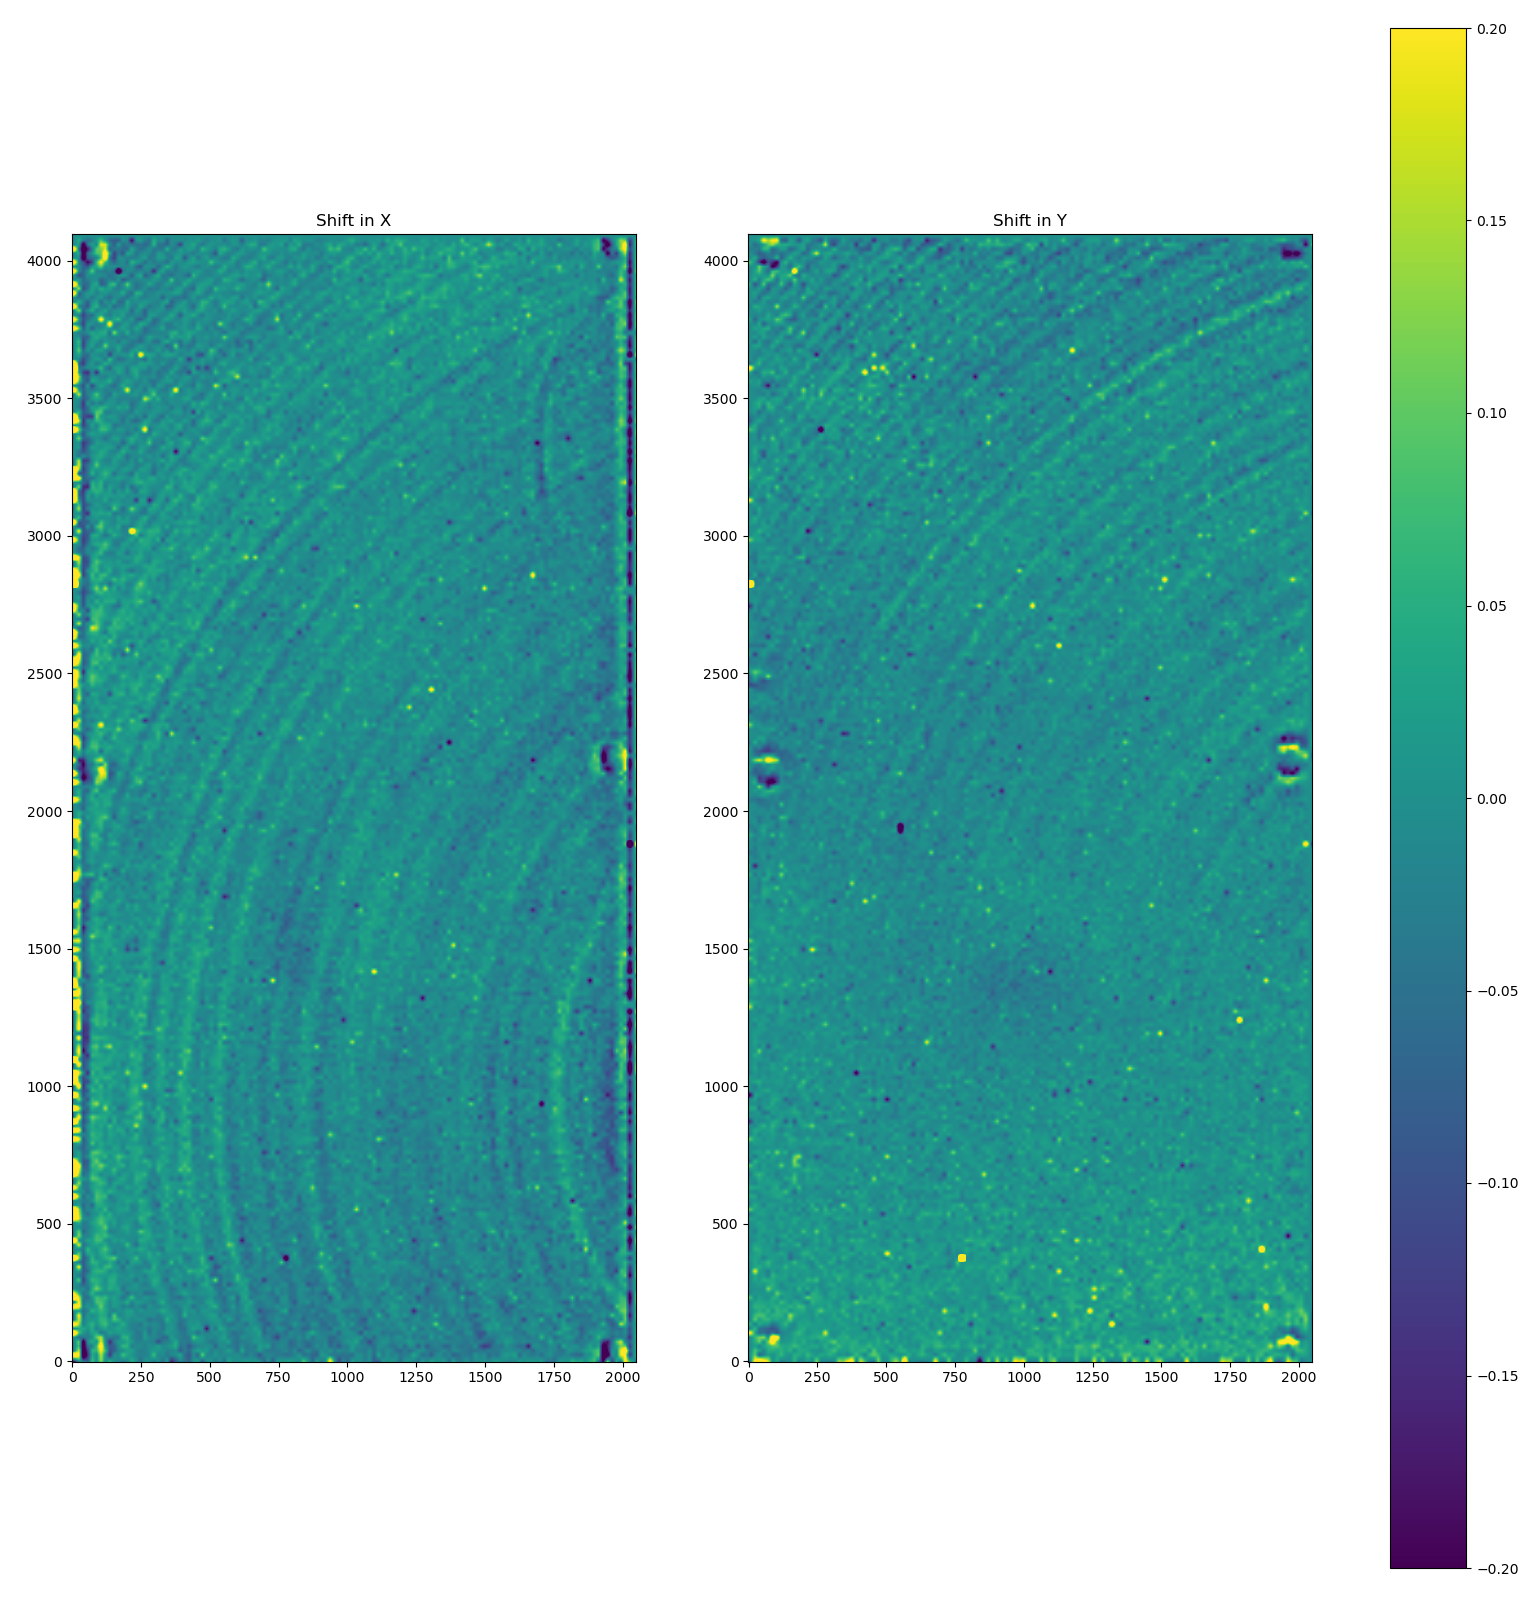
\includegraphics[width=0.5\textwidth]{plots/ringmaps.png}
    \caption{A visualisation of the CCD distortions caused by silicon tree rings, tape, etc. The axes are the pixels in the CCD. The left plot represents the shift in the x-direction, and the plot on the right represents the shift in the y-direction. The distortions shown are found by extracting the sources present in the Gaia catalogue per CCD per filter, then avergaing their shift between their positions in the Gaia catalogue and the Legacy catalogue.}
    \label{fig:ringmaps}
\end{figure}

Our initial step involved creating a distortion map for each CCD in the DECam instrument. The distortion maps were generated by averaging the differences between Legacy measurements and their expected values from the Gaia catalog. Figure \ref{fig:ringmaps} illustrates the distortions of a single CCD applied to a smooth mesh, with distinct plots for distortions along the x-axis and y-axis. The color scale ranges from black/purple (-0.2 pixels) to yellow (+0.2 pixels), providing a visual representation of the magnitude of distortions across the CCD. 

Figure~\ref{fig:dcr} shows the offsets of Gaia stars along the direction to the zenith, before and after the DCR correction \todo{state number of bricks / measurements used}. As expected from Equation~\ref{eq:dcr}, before correction the offset grows with airmass and with the colour difference from the reference stars, and it has opposite signs for stars redder ($c > 0$) and bluer ($c < 0$) than the reference. Stars with colours close to the reference colour ($c \approx 0$) are barely displaced. After correction, the trend is largely removed, with small residuals remaining at the highest airmasses.

\begin{figure}
    \centering
    % 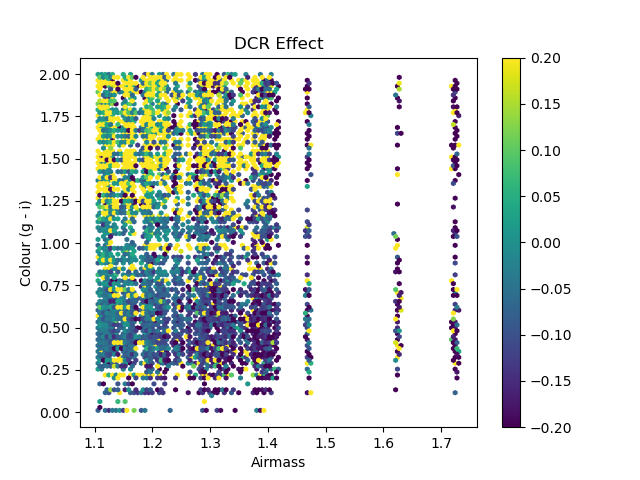
\includegraphics[width=0.5\textwidth]{plots/DRC.png} % old version: absolute g-i, no units on colourbar
    \figtodo{DCR before/after: hexbin of median offset along $\hat{\mathbf{p}}$ (arcsec) vs.\ airmass and relative $g-i$ colour, $r$ band, two panels. Slide 15; run/dcr-plots.ipynb.}
    \caption{Median offset of Gaia stars along the direction to the zenith in the $r$ band, as a function of airmass and relative $g-i$ colour, before (top) and after (bottom) the DCR correction of Equation~\ref{eq:dcr} \citep{Bernstein_2017}. Before correction, stars redder and bluer than the astrometric reference stars are displaced in opposite directions, by amounts that grow with airmass. After correction, this trend is removed.}
    \label{fig:dcr}
\end{figure}

The combined effect of all three corrections on the positional accuracy of Gaia stars is shown in Figure~\ref{fig:scatter_vs_mag} and discussed in Section~\ref{sec:corr_analysis}.


% TODO delete or include?: Unfortunately, these corrections only apply on the small scale. For stars that have way-off proper motions measured by the Legacy data, 


%% TODO Discussion section
% extended DCR, did RM differently; why? 
% They tried paramatric and still had residuals -- might as well get maps from data
% we are more interested in correcting than understanding the phenomena


\newpage
\clearpage


% \section*{Future Work: CHORD FRB Population Modelling}

% This section outlines my future plans after the transition from a Master's program to a Ph.D., with a specific focus on contributing to the Fast Radio Burst (FRB) population modeling project within the CHORD collaboration. The proposed Ph.D. research aims to address several crucial components, including flux calibration, Radio Frequency Interference (RFI) flagging, the development of a real-time FRB search pipeline, and the implementation of data injection techniques to assess the efficiency of the search process.

% \subsection*{Fast Radio Bursts and CHORD}

% First discovered in 2007 \citep{lorimer2007}, Fast Radio Bursts (FRBs) are transient and intense bursts (up to $10^{44}\text{erg s}^{-1}$) of radio frequency signals lasting only a few milliseconds, with extragalactic and cosmological origins currently observed in the redshift range $z\sim 0.03$ to $z\sim 1$ \citep{ng2023brief}. These events occur at an estimated all-sky rate of $\sim 5000$ per day at CHIME/FRB’s sensitivity \citep{ng2023brief, CHIMEAmiri_2021}.

% The majority of Fast Radio Bursts (FRBs) are isolated occurrences, but a small fraction exhibit repeating patterns. Currently, 51 repeating FRBs have been published, with more awaiting publication \citep{ng2023brief}. Analysis of 46 repeating FRBs in the \cite{CHIME2023updating} study reveals that they often cluster in time and energy distribution, exhibiting periods of heightened activity followed by quiescence. The first CHIME/FRB catalog \citep{CHIMEAmiri_2021}, comprising over 500 FRBs, provides a foundational dataset for population analysis, revealing different patterns in the frequency-vs-time plane between repeaters and non-repeaters.

% The question of whether one-off FRBs represent cataclysmic events or are simply undetected repeats remains unanswered \citep{ng2023brief}. One FRB has been definitively linked to a magnetar in our Milky Way, reinforcing the magnetar model. However, the diversity of FRB properties, such as periodic activity seen in some cases, challenges a universal explanation. While nearly 40 FRBs have host galaxies identified, no conclusive progenitor associations have been established, making the study of FRB host environments an ongoing challenge. Recent analyses suggest FRBs can originate from various types of host galaxies, challenging earlier assumptions about their origins \citep{ng2023brief}.

% CHORD, the Canadian Hydrogen Observatory and Radio-transient Detector, is a proposed radio telescope designed for the study of various processes within its observation window spanning from $300$ MHz to $1500$ MHz. These processes include examining neutral hydrogen in nearby galaxies via the 21-cm spin-flip transition, conducting cosmological intensity mapping of the 21-cm signal, exploring pulsar science, and investigating Fast Radio Bursts (FRBs). In comparison to CHIME, CHORD boasts greater sensitivity within a more compact field of view and offers a broader wavelength coverage. Consequently, CHORD is anticipated to detect more FRBs, and for each detection, it will provide more extensive wavelength coverage. Additionally, CHORD facilitates the connection of FRB observations conducted with other telescopes, primarily in the $1.4$-GHz band, with CHIME’s lower-frequency band, thereby extending the observational band down to $300$ MHz \citep{chord2019}.

% CHORD's unique design, with its phased-array feed technology and high-precision time-sampling, will enable the telescope to measure the pulse shapes and polarization properties of FRBs with unprecedented precision. This detailed information will be used to infer the physical processes behind FRB emission and to model the distribution and properties of FRB sources across the cosmos. 
% CHORD's sensitivity and resolution will also allow it to detect weaker FRBs and to identify FRBs with unusual properties, such as dispersion measures and pulse widths. These discoveries will further our understanding of the FRB phenomenon and provide constraints on FRB progenitors \citep{chord2019}.


% \subsection*{Research Objectives}

% In the pursuit of this Ph.D., the primary objectives encompass a comprehensive exploration of key aspects of FRB research. The first objective focuses on the development of robust algorithms for Radio Frequency Interference (RFI) flagging. These algorithms will be designed to remove strong outlying values in the data stream that might be mistaken for FRBs, and may incorporate machine learning approaches to improve the accuracy and efficiency of RFI identification, particularly in the context of dynamic and evolving RFI patterns.


% The CHIME RFI transform chains are intricate systems designed for efficient mitigation of interference in the intensity data stream. Comprising over 100 transforms, the subpipeline employs a sequence of clipping and detrending operations to mask RFI \citep{CHIME_RFI_2023}. The process is iterative, aiming to recognize and suppress RFI-induced statistical outliers incrementally, thus maintaining the integrity of the intensity probability distribution function. The clipping transforms, including static masks and dynamic outliers elimination, are nested within a detrending transform chain, addressing large-scale variations caused by factors like RFI, forward gains, and digital beamforming. Polynomial and spline detrenders are utilized in this chain, working in conjunction with the clipping transforms to generate masks for downsampled intensity chunks. Additionally, an auxiliary transform chain is proposed as a dynamic adaptation to unforeseen RFI events, such as "RFI storms." This chain, with a cautionary approach, operates along the frequency axis, expanding the mask to suppress RFI residuals while minimizing potential biases. The CHIME RFI transform chains are empirically configured for optimal performance, demonstrating a robust methodology for real-time RFI mitigation in intensity data streams \citep{CHIME_RFI_2023}.

% In developing the CHORD RFI system, I would leverage the foundational principles of the CHIME RFI system while acknowledging the need for significant modifications tailored to CHORD's unique characteristics. Given that the CHIME RFI system was hand-tuned for the CHIME telescope based on early CHIME-pathfinder data, I would adopt a similar iterative approach for CHORD, accounting for its wider frequency range and distinct "deep-dish" design with a narrower field of view. CHORD's design, with its focused observation and reduced susceptibility to RFI due to the narrower field of view, presents an advantage over CHIME, which has a broad field of view extending almost horizon-to-horizon. The RFI mitigation strategy for CHORD would involve adapting and refining the CHIME RFI transform chains, incorporating the lessons learned from CHIME's hand-tuning process, and addressing the specific challenges posed by CHORD's unique telescope design and broader frequency range. This approach ensures a robust and tailored RFI system for CHORD, optimizing its performance for radio observations in diverse and challenging environments.

% The second objective involves contributing to the design and implementation of a real-time FRB search pipeline capable of processing large volumes of data promptly, which the team at Perimeter Institute are working on. The optimization of algorithms for the rapid detection and localization of FRBs is critical to ensuring a timely response and facilitating subsequent follow-up observations.

% The third objective revolves around data injunction techniques to evaluate the FRB search pipeline's efficiency. Metrics and tools will be developed to assess factors such as sensitivity, false positive rates, and computational performance. Additionally, the interplay between RFI flagging and the search pipeline will be explored to refine the overall FRB detection process.


% The CHIME/FRB injection system is a multifaceted structure comprised of several components \citep{CHIME_injection_2023}. It includes an application program interface (API) named "mimic," an injections database for managing injection statuses, and an injection "driver" responsible for systematically injecting synthetic pulses. Notably, the system duplicates the live CHIME/FRB data stream, injecting simulated pulses into the replicated data to prevent interference with the live stream. The injection system operates within a Docker stack on the CHIME/FRB analysis cluster, employing OS-level virtualization for standardized runtime environments. The Injection API, orchestrated by mimic, manages real-time injections by interacting with L1 nodes via RPCs. The system involves the InjectionDriver, which organizes injection requests by reading an hdf5 file containing a population of generated FRBs. The Injection Database, hosted on the CHIME/FRB archiver, stores injection and detection parameters. The InjectionSnatcher module in the L2/L3 pipeline flags injections as detected or not detected based on metadata analysis, with a focus on matching arrival times and dispersion measures. This comprehensive architecture ensures efficient and controlled injection of synthetic pulses for testing and calibration purposes in the CHIME/FRB system \citep{CHIME_injection_2023}.


% In designing the injection system for CHORD, the initial approach will draw inspiration from the successful CHIME model. However, recognizing the challenges faced by the "injection snatcher" approach in CHIME, we plan to implement a more careful and controlled method. A key deviation involves meticulous tagging of injected data as it progresses through the real-time detection system. This intentional tagging will allow us to distinguish and isolate the injected data from the live data stream. The primary objective is to establish a clear separation between injected and live data, mitigating potential interference issues. This modification not only aims to address the difficulties encountered with the CHIME injection snatcher but also facilitates continuous real-time injections. The goal is to systematically map out the time-varying aspects of the entire FRB system's detection sensitivity, enabling comprehensive and ongoing calibration efforts. This strategic adjustment in the injection system design for CHORD emphasizes precision, control, and a continuous monitoring capability to enhance the understanding of the system's performance over time.


\clearpage
\newpage

\bibliography{mybib}

\bsp	% typesetting comment
\label{lastpage}
\end{document}

